\documentclass[12pt]{article}

\usepackage{amsmath, amssymb, amsthm}
\usepackage{graphicx}	% use to include graphics
\usepackage{verbatim}
\usepackage{multicol}

\makeatletter
\renewcommand\section{\@startsection{section}{1}{\z@}%
								 {-3.5ex \@plus -1ex \@minus -.2ex}%
								 {2.3ex \@plus.2ex}%
								 {\normalfont\large\bfseries}}
\makeatother

\title{CSE 490h Assignment 4}
\author{
Colin Scott and Bill Cauchois \\
}

%%%%%%%%%%%%%%%%%%%%%%%%%%%%%%%%%%%%%%%%%%%%%%%%%%%%%%%%%%%%%%%%%%%%%%%%%%%%%%%%%%%%%
\begin{document}
\maketitle

\section{Design Decisions}

\subsection{Heartbeats and Leader Election}

Every \emph{heartbeat period}, each manager node sends out a heartbeat message to every other
node to determine if that node is alive (upon receiving such a message, the other node is
obligated to respond; like with a ping). The result of such a \emph{heartbeat round} is that
every node knows which nodes are up. We call this set of `up nodes' with respect to the node
sending the heartbeat messages the \emph{alive set}. Usually, every node will have the same
alive set (unless messages are dropped).

Given this alive set, leader election is performed using a simple algorithm. The node in the
\emph{alive set} with the lowest address is designated the leader. That is, the leader is always
the Paxos node with the lowest address.

However, taking into account the unreliability of the transport medium, it is possible that
(due to some messages being delayed or dropped) more than one node will think that it's the
leader. This is OK, since safety is ensured by Paxos.

Additionally, if any node receives a message from a node whose address is not in its alive set,
it automatically adds that node to its alive set.

\subsection{Client Redirects}

Although (in the best case) every node in the Paxos group will know who the leader is, it is not
always the case that the clients know who the leader is. Since commit attempts are sent to the leader,
we have implemented a system of `RPC redirects' to ensure that the client's commit attempt ends up in the right place.

A client may send its commit attempt to any node in the Paxos group. If that node is \emph{not} a leader,
it will respond with a forward message telling the client that it should retry its request at node $n$,
the leader of the Paxos group. On the other hande, if the original node is the leader, then the commit may
proceed normally.

\subsection{Syncing Newly Elected Servers}

With multi-paxos, when a new leader is elected, he needs to know which Paxos instances have been chosen
so that he can choose a new Paxos instance ID when he starts a transaction commit. We call this process
\emph{syncing} or `getting the servers up to speed'.

Our algorithm for syncing isn't perfect -- we only manage to learn the most recently \emph{learned}
values, not the most recently \emph{chosen} values. This is OK though, since Paxos ensures safety in all
cases. It's only a performance optimization to get the newly elected leader up to speed.

\subsection{Gaps in Paxos}

Due to the nature of our system, a value must be chosen for each consecutive instance of Paxos. For example,
it is not possible to have Paxos instances 1, 2, and 4 chosen -- but not 3. Sometimes we do wish to skip a
number though, and in that case we propose and then choose a \emph{NOP}, or no-op.

It's the job of the learner role to fill gaps in the Paxos instance by proposing a NOP when there has been no
progress for a while. This ensures that pending transactions will eventually be committed.

\subsection{Write-Through Cache Coherence}

We maintained our write-through cache coherence from project 3 so that we wouldn't have to reinvent the wheel. In the end, only two changes to the client were required:

\begin{enumerate}
\item
    Whenever a client receives a response with the \textsc{ForwardTo} field set, it will
    redirect its RPC to another Paxos server.
\item
    Clients generate a unique transaction id for each new transaction. This is to ensure
    that no transaction gets executed twice by Paxos -- if a paxos node recieves a commit
    attempt with an id that has already been executed, we immediately return the result
    to the client rather than executing the transaction twice.
\end{enumerate}

\subsection{Two Phase Commit/Multi-Paxos}

We originally planned to implement primary-backup replication since it seemed easier to reason
about. In re-reading the replication paper however, we realized that the complexity cost of
this approach far outweighed its benefits. In particular:
\begin{enumerate}
\item
    For synchronous replication, two-phase commit is required for propagating updates
    to the replicants.
\item
    Deciding when a lease has expired is non-trivial, since there is no global clock. 
\item
    In lecture Tom seemed to indicate that PAXOS could simply choose the primary for the
    next round -- In fact, PAXOS must choose the entire ‘epoch set’ (the set of all replicants)
    each round. This is because 2PC is a blocking protocol; if any of the replicants is down,
    the primary will not be able to make progress. We would already have to implement
    heartbeats for PAXOS anyway, so it seemed redundant to have PAXOS also decide on the
    set of running replicants.
\end{enumerate}

\section{Questions}

\noindent \textbf{(a)}
In your design, how is callback state maintained? Do the servers vote on changes to the
callback state using Paxos, do they elect a leader to centralize the callback state,
or do you use some other mechanism? Is it even necessary for correctness or performance
that the server callback state be consistent with the state of the client caches?

No.  Invalidates are simply an optimization -- if a client tries to commit a transaction
that depended on out-of-date files, the Paxos servers will refuse to commit the transaction.

Caching certainly helps performance though, since in the common case clients don’t need to
flush their caches between or within transactions.

\noindent \textbf{(b)}
In your design, how is storage state maintained? Does every server participating in Paxos 
store every modification of every file, do they elect a primary/backup, or do you use
some other mechanism?

We chose to implement state-machine replication such that every Paxos server (eventually)
executes every transaction. Paxos ensures that there is a global order of transactions
applied at each paxos node, and that any newly elected server can eventually get up to
speed with the global order. In every case, safety is preserved by Paxos % BITCHES

\section{Synoptic}

We defined the following events to model the paxos roles' behavior:

\begin{enumerate}
\item Proposer
    \begin{enumerate}
        \item \textsc{NEW-PROPOSE}
        \item \textsc{RECV-PROMISE}
     \end{enumerate}
\item Learner
    \begin{enumerate}
        \item \textsc{RECV-ACCEPTED}
        \item \textsc{LEARNED-VALUE}
    \end{enumerate}
\item Acceptor
    \begin{enumerate}
        \item \textsc{IGNORE-PREPARE}
        \item \textsc{ACCEPT-PREPARE}
        \item \textsc{ACCEPT-ACCEPT}
        \item \textsc{IGNORE-ACCEPT}
    \end{enumerate}
\end{enumerate}

Here's what our final synoptic graph looked like, which corresponded roughly to what
we expected:

\begin{center}
    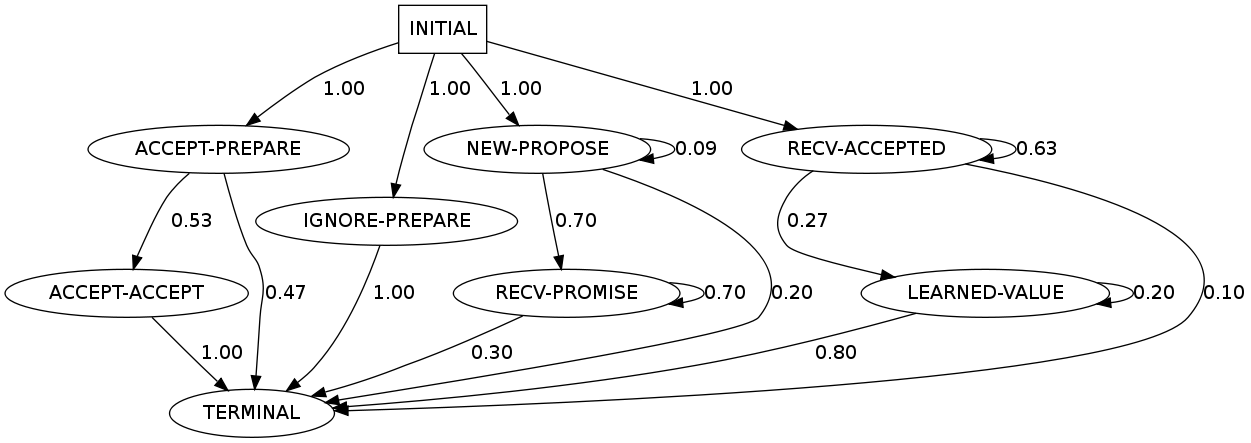
\includegraphics[width=500px]{synopticOutProj4.png}
\end{center}

You'll notice that we separated the state machine for each paxos role out. In
doing so, we actually lose some information, since the state transitions for
a given state machine may depend on the states of the others. For example,
when a proposer fails to recieve promises from a majority of acceptors, it may be because
the acceptors have crashed, or it may be because they have already promised
not to accept proposals numbered less than n (in which case the acceptor state
will transition to IGNORE-PREPARE).

I originally tried to define a single state machine that included all roles in
the system to encapsulate these dependancies, but the result was totally non-sensical. In talking to Ivan, we
came up with two alternatives that might encapsulate the desired information:

\begin{enumerate}
\item A cross-product state machine, where each state in the final synoptic
output graph encapsulates the state of each of the individual paxos roles in
the system. This would require global information about the states of each of the nodes
\item An infinite state machine, where information about the proposal
/numbers/ is encapsulated in the states of the paxos roles. This way we could
"trace" the progress of a given proposal across different roles. But because
the state machine is inifite, there is really little point in using Synoptic
anymore -- synoptic excells at /compressing/ graphs, and with an infinite
state machine the output is ultimately just a uncompressed /visualation/ of the log.
\end{enumerate}

Honestly, synoptic was quite difficult to reason about and get working
correctly. (I had a conversation about
this with Ivan.)

\end{document}
